% arara: pdflatex: { draft: true, shell: yes }
% arara: biber
% arara: pdflatex: { synctex: true, shell: yes}    
% arara: pdflatex: { synctex: true, shell: yes}
\documentclass[american, hauptseminar, twoside]{zihpub}

\usepackage[hidelinks=true]{hyperref} 
\usepackage[backend=biber,style=numeric]{biblatex}
\usepackage{import}
\usepackage{color}
\usepackage{here}
\usepackage{minted}
\usepackage{csquotes}
\usepackage{graphicx}
\usepackage{pgfplots}
\usepackage{tikz}

\usepackage{caption}
\usepackage{subcaption}

\definecolor{tudblue}{RGB}{0,89,163}
\definecolor{tudgreen}{RGB}{0,122,71}
\definecolor{tudorange}{RGB}{232,123,20}
\definecolor{codebg}{rgb}{0.97,0.97,0.97}

\addbibresource{refs.bib}
	

\author{Tobias Frust}
\title{Adapteva Parallella: Crowd-funded Low-budget Open-source HPC}
\matno{3749068}
\betreuer{Ronny Brendel}

\begin{document}
	\section{Introduction}
		Beginning in 1971, when the first commercial microprocessor was released, to 2003, performance improvements have mainly been accomplished by increasing the clock frequency. By boosting the clock frequency, heat dissipation increases as well. This is why that measure is not applied anymore and the clock rate remained static. Hardware developers needed to find different ways how to speed up their processors. The solution was to integrate more than one processor on a chip. Nowadays, any device, be it a desktop pc, a laptop or a smartphone, has a multi-core CPU architecture. Attempts to achieve better speed resulted in various design methodologies. For this reason, parallel programming is necessary to exploit the maximum performance, whereas in the past, implementations increased their performance with every processor generation due to their serial speedup. 
		\\
		In this work, the Adapteva Parallella, a crowd-funded low-budget open-source High-Performance Computing (HPC) Platform, is presented. In Section~\ref{sec:parallella} the history of the company Adapteva is presented. Furthermore, the architecture and characteristics of that board are introduced with a special focus on the Epiphany coprocessor.
		Section~\ref{sec:implementation} shows how to implement the one-dimensional Fast Fourier Transform (FFT) on the Epiphany processor. A special focus will be the data transfer from host to device. Finally, the performance of this implementation will be measured.
		In Section~\ref{sec:gpu} the Epiphany chip is compared to another many-core architecture: NVIDIA's Maxwell GPU architecture. To stay fair, the comparison is based on energy efficiency with respect to chip area. The last section will summarize the results and assesses the Parallella's potential as a HPC platform.
		
		\clearpage
	\section{Adapteva Parallella}
		\label{sec:parallella} 
		In this section Adpatava's company history and its Parallella board are presented. Furthermore, the architecture of the Epiphany chip is shown.
		\subsection{Company History}
			Adapteva was founded on February 2008 with the goal to develop and build the world's most energy efficient microprocessor chips and single board computers. A few months later in October, the first prototype layout of Epiphany core was completed. The tape-out of the Epiphany-I prototype in 65 nm structure width was in June 2009 and they were able to secure a 1.5M US \$ Series-A funding from Bittware. Release of the first product, the Epiphany-III 65nm 16-core chip, was in May 2011. Tape-out of the first 64-core version in 28 nm structure width was in August 2011 and in the same year Adapteva reached break-even as a company. One year later in August, 50 GFLOPS/Watt energy efficiency could be demonstrated with the sampled product.
			The Parallella Kickstarter project was launched in October 2012 and the first prototypes were shipped by the end of the year. Dispatch of the Parallella Board to the Kickstarter backers began in July 2013 and was finished in April 2014.~\cite{Adaptev2015}
			
		\subsection{Parallella Kickstarter Program}
			On September 28, 2012 Adapteva launched the Parallella Kickstarter project. They were asking for help, because getting corporations to buy into parallel computing has proven challenging. Based on this knowledge they said, that the only way to create a sustainable parallel computing platform is a broad movement. 
			\\
			The goal was to implement a design that is based upon the following principles~\cite{Adaptev2012}:
			\begin{itemize}
				\item \textbf{Open Access:} no special access or non-disclosure agreements (NDA) shall be necessary. All architecture and SDK documents shall be available online.
				\item \textbf{Open Source:} Parallella platform shall be based on free and open-source development tools. All board design files will be open-source once the Parallella board is released.
				\item \textbf{Affordability:} The Parallella board shall not cost more than 100 \$. The barrier for customers, who want to develop high performance applications, shall be removed.
			\end{itemize}
			They wanted to democratize access to parallel computing, close the knowledge gap in parallel programming and build the most energy-efficient computing architecture. The Kickstarter project gained 898,921\$ from 4,965 backers. Basis of the Parallella board was the Epiphany chip, developed by Adapteva since 2008~\cite{Adaptev2012}.
		
		\newpage
		\subsection{Parallella Board}
		The Parallella board was released during a Kickstarter project and is presented in the next section.
			\subsubsection{General Overview}
				The Parallella board is a credit card-sized, high performance computer based on Adapteva's Epiphany multi-core chips (Figure~\ref{fig:board}).
				\begin{figure}[H]
					\begin{center}
						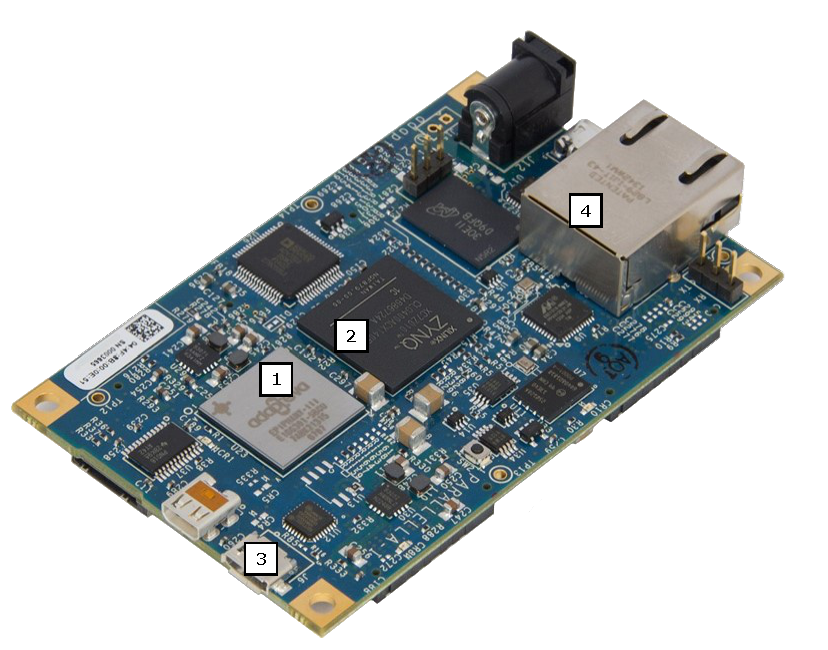
\includegraphics[width=0.9\textwidth]{grafiken/board.pdf}
						\caption{The Parallella Board \cite{Parallell2014}.}
						\label{fig:board}
					\end{center}
				\end{figure}
				The main elements of this board are the dual-core ARM Cortex A9 host processor~(2) and the 16-core Epiphany coprocessor~(1). It includes one Gigabyte RAM, Gigabit Ethernet~(4) and a micro SD card~(3) as storage. The operating system is Linux, e. g. Ubuntu. The Epiphany chip has a peak performance of 26 GFLOP/s in single-precision, and has an energy consumption of two Watts.
				Figure~\ref{fig:sysoverview} shows the system overview of the Parallella. It consists of two parts, the Zynq host processor with a dual-core ARM A9, and a programmable logic. This FPGA is a configurable interconnect network, which is the connector between the host and the Epiphany coprocessor. This example shows the configuration with 64 cores. The interconnection bandwidth from ARM dual-core to the Programmable Logic is denoted with 2.4 GB/s, and between Epiphany and programmable logic 1.4 GB/s. Later in this work the transfer bandwidth will be examined in detail (Section~\ref{sec:bandwidth}).
				\begin{figure}[H]
					\begin{center}
						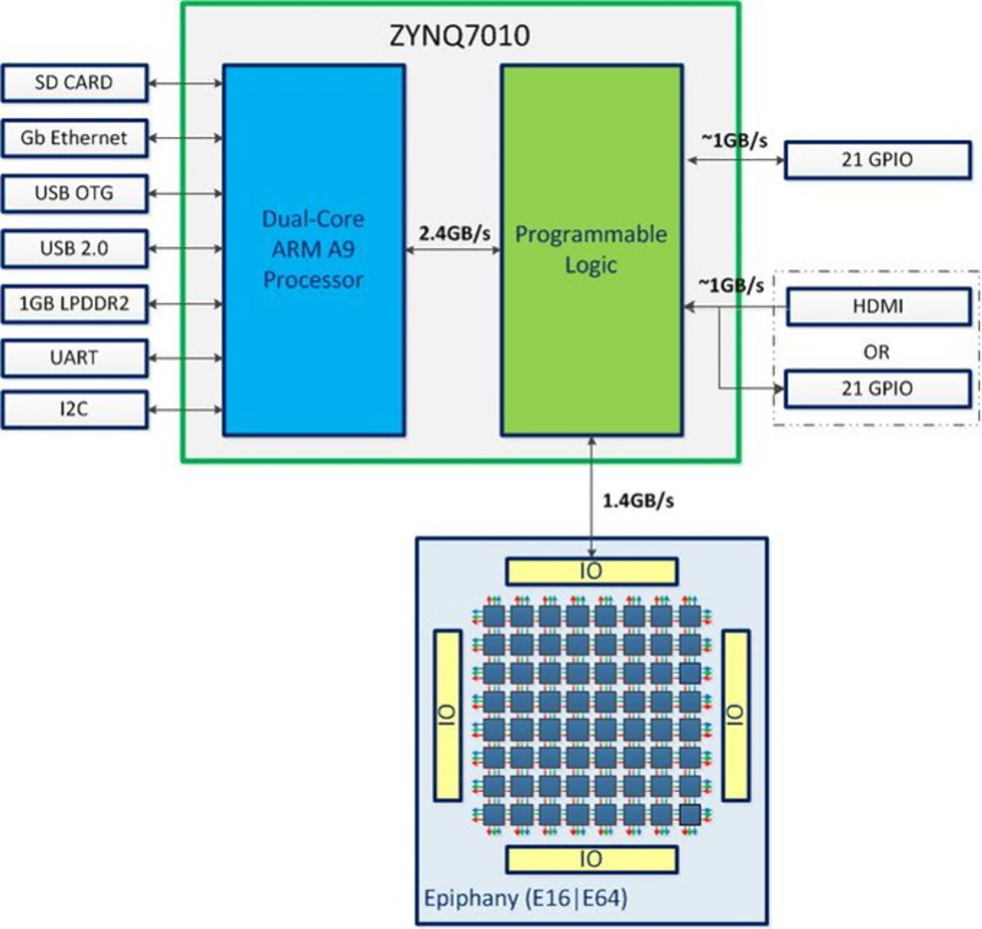
\includegraphics[width=0.9\textwidth]{grafiken/sysoverview.pdf}
						\caption{System overview of the Parallella Board~\cite{Adaptev2015a}.}
						\label{fig:sysoverview}
					\end{center}
				\end{figure}
			\subsubsection{Epiphany Architecture}
				Adapteva assumes that current architectures are hitting a wall and that the future of computing is parallel and heterogeneous \cite{Adaptev2015a}. Therefore the Epiphany architecture, which serves as coprocessor to ARM or Intel CPUs, was released. Figure \ref{fig:epiphany} shows the system overview of the 64-core version of the Epiphany chip. The cores are arranged in a quadratic mesh. Any core is only connected to its direct neighbors in east, south, west and north direction. Each processing element is a RISC design with in-order execution. It consists of one integer ALU, a floating-point unit with support for fused multiply-add and a 64-word register file. Every core has its own local memory to store program and data in. The size of this memory is limited and amounts in 32 Kilobytes per core in case of the 16-core Epiphany. It is separated into four eight KB memory banks. For this reason, those resources need to be treated carefully and data partitioning is necessary. Optimal performance can only be achieved if data is placed in local memory. The Epiphany chip features a magic address translation, which means, that any core can access all memory locations, be it transfers to DRAM, other cores or off-chip. 
				\begin{figure}[H]
					\begin{center}
						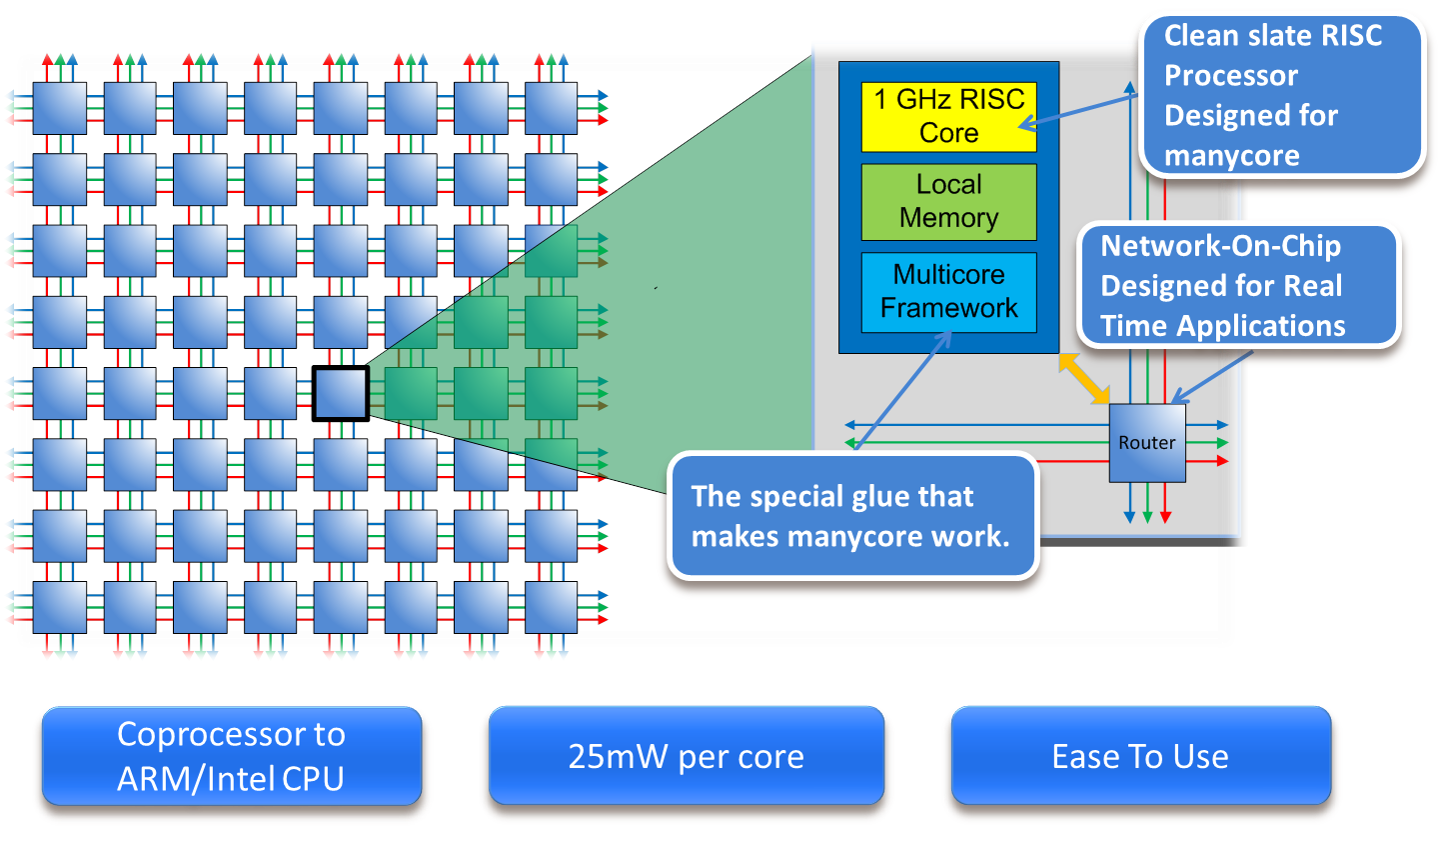
\includegraphics[width=0.9\textwidth]{grafiken/epiphany.pdf}
						\caption{The Epiphany Architecture~\cite{Adaptev2015a}.}
						\label{fig:epiphany}
					\end{center}
				\end{figure}
				
				\paragraph{eMesh Network on Chip}\mbox{}\\
					All Epiphany cores are connected by a 2D mesh topology with only nearest neighbor direct connections in east, south, west and north, that is called eMesh Network on Chip. Figure~\ref{fig:emesh} shows the structure of this network. There are three separate mesh structures, that serve different types of transactions. The \textit{cMesh} is used for on-chip write transactions. Its maximum bidirectional throughput is eight bytes/cycle in each direction. The \textit{rMesh} is used for all read requests. The maximum throughput is one read transaction every eight clock cycles in each routing direction. The \textit{xMesh} is used for off-chip write transactions and for passing through transactions destined for another chip in a multi-chip system. The maximum throughput depends on the available off-chip I/O bandwidth.
					\begin{figure}[h]
						\begin{center}
							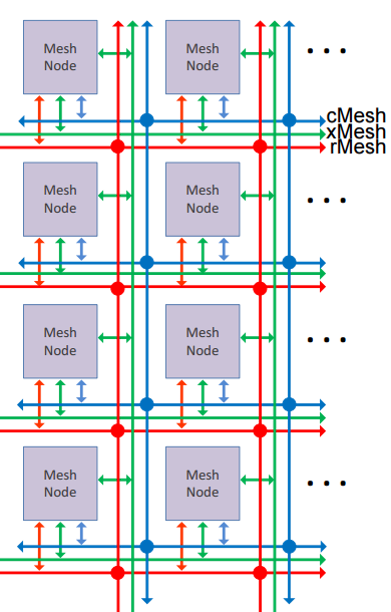
\includegraphics[width=0.27\textwidth]{grafiken/emesh.png}
							\caption{Structure of the eMesh Network on Chip~\cite{Adaptev2011}.}
							\label{fig:emesh}
						\end{center}
					\end{figure}
					Write transactions move through the network with a latency of 1,5 cycles latency per hop. In a 64-core configuration the connection from the left to the right edge would thus take twelve clock cycles. The \textit{cMesh} has lower latency than the \textit{xMesh}. This is why tasks with significant inter-core communication should be placed together on the same chip for better performance~\cite{Adaptev2011}.
					\\
					Furthermore, write transaction are optimized over read transactions. Writes are approximately 16 times quicker than reads for on-chip communication. The network is free of deadlocks, because of the separation of read and write meshes together with a fixed xy-routing scheme. The network can be scaled to very large arrays, it is only limited by the size of the address space~\cite{Adaptev2011}.
					
					\clearpage
	\section{One-Dimensional Fast Fourier Transform}
		\label{sec:implementation}
		\begin{figure}[b!]
			\begin{center}
				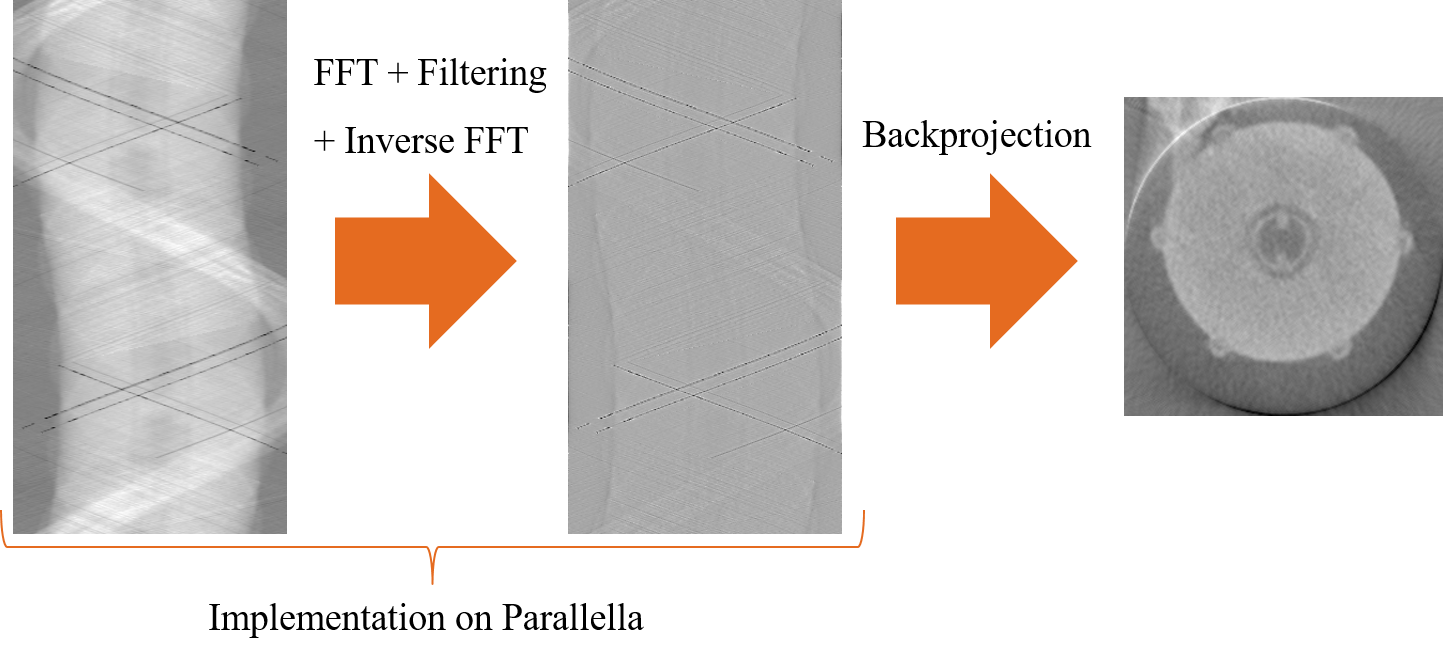
\includegraphics[width=\textwidth]{grafiken/fbp.png}
				\caption{Principle of the Filtered Backprojection Algorithm.}
				\label{fig:fbp}
			\end{center}
		\end{figure}
		In the course of this work the one-dimensional Fast Fourier Transform (FFT) is implemented and parallelized on the Parallella board. The FFT is a very important algorithm in many fields, e.g. signal processing. The filtered backprojection is an algorithm to reconstruct images from projections. In computed tomography, there are rays traversing a measurement field from the source to the detector. The detector measures the intensities of the rays after interacting with the measurement area. To obtain the original image it is reconstructed from the set of projections. As Figure~\ref{fig:fbp} shows, the filtered backprojection consists of two parts: filtering and backprojection. Filtering can be realized in two different ways. The first possibility is to convolute with the filter function in time domain. The second approach is to convert a signal from the time domain to a representation in the frequency domain via the FFT. Then, the signal can be multiplied with the filter function element-wise. Next, it needs to be reconverted via the Inverse FFT. To obtain the measured cross-section it finally needs to be back-projected. 
		\\
		In this section it will be shown how the FFT is implemented and parallelized on the Parallella board. Finally, performance measurements will be presented.
		
		\subsection{Implementation}
		\begin{figure}[h]
			\begin{center}
				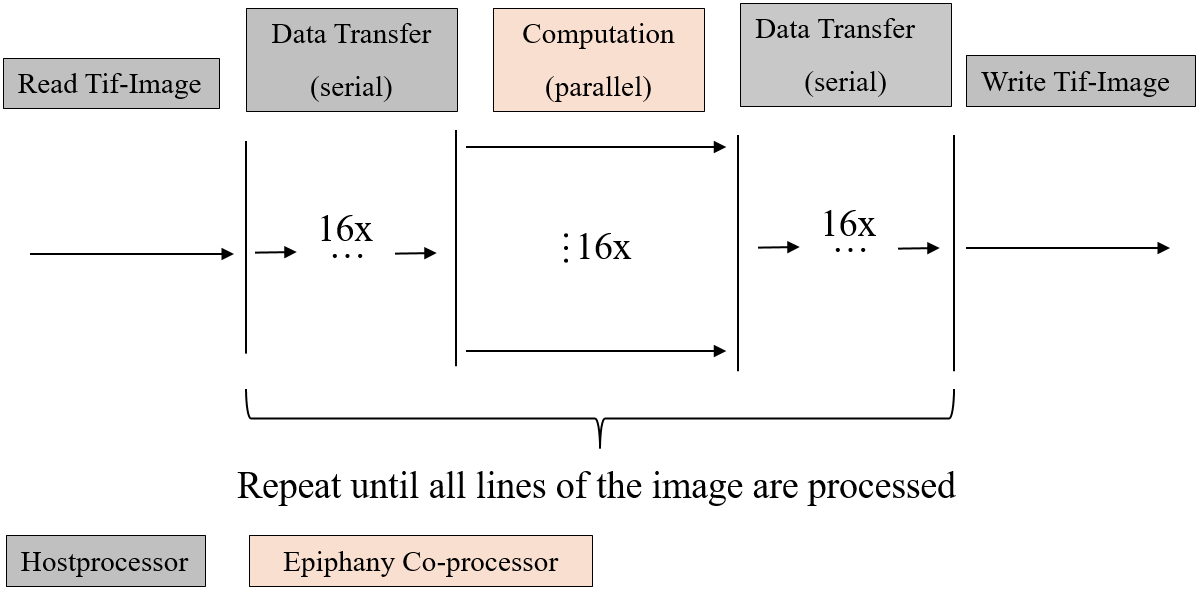
\includegraphics[width=\textwidth]{grafiken/implementation.png}
				\caption{Workflow of the filtering procedure.}
				\label{fig:implementation}
			\end{center}
		\end{figure}
			The FFT is a widely used algorithm, thus it makes sense to examine its performance on this architecture. The implemented program works as shown in Figure~\ref{fig:implementation}. The input data is stored as TIF image. The first step is to read the image. For this, the so called \textit{LibTiff}-Library \cite{Warmerdam2015} is used. Once, the data is in main memory, it can be transfered to the local memory of each used Epiphany core. Since the chip contains 16 cores, there are 16 memory transfers from host to device memory. Each transfer copies two lines of the image to the Epiphany. Then, the parallel computation can start. The first step is to calculate the Fast Fourier Transform of each line. Every element is multiplied with the filter function. Finally, the inverse FFT converts the data back to the domain domain. Once the computation is finished, the data is transferred back from local memory to the main memory. Via the \textit{LibTiff}-Library \cite{Warmerdam2015} the filtered data is written back to the TIF files.
			
			
		\subsection{Optimization}
		\label{sec:bandwidth}
					To run an application on the Epiphany device you need to initialize it. Figure~\ref{code:init} shows how this is done. The first step is to reset the Epiphany device. Afterwards, a workgroup needs to be opened (line~5) and finally the executable needs to be loaded into the group (line~11). The next step is to copy data from host memory to the local memory of each core. Once copying is finished, computation can start. Due to the limited amount of per-core local memory, only few image lines can be computed in parallel. Copying and computation has to be repeated, until the whole image is computed. In a first approach this could be realized by repeating the whole initialization procedure again, but this is very time consuming.
					\\
					This is why it is realized differently. The Epiphany is started only once and runs in continuous loop. Any time, data copy is finished, the Epiphany gets a signal, that computation may start. Without this intuitive approach the hardware could not be utilized efficiently.
					\begin{figure}[h]
						\inputminted[bgcolor=codebg,
						linenos=true,
						frame=lines,
						numbersep=5pt,
						fontsize=\footnotesize,
						breaklines=true,
						tabsize=4]{c}{code/init.c}
						\caption{Initialization procedure of the Epiphany device}
						\label{code:init}
					\end{figure}
				\paragraph{Optimization of Data Transfer}\mbox{}\\
						During the process of implementation and optimization a severe bottleneck was identified: the data transfer. Figure~\ref{fig:circle} shows the portion of the computation part versus the portion of the read and write part.
						\begin{figure}[h]
							\centering
							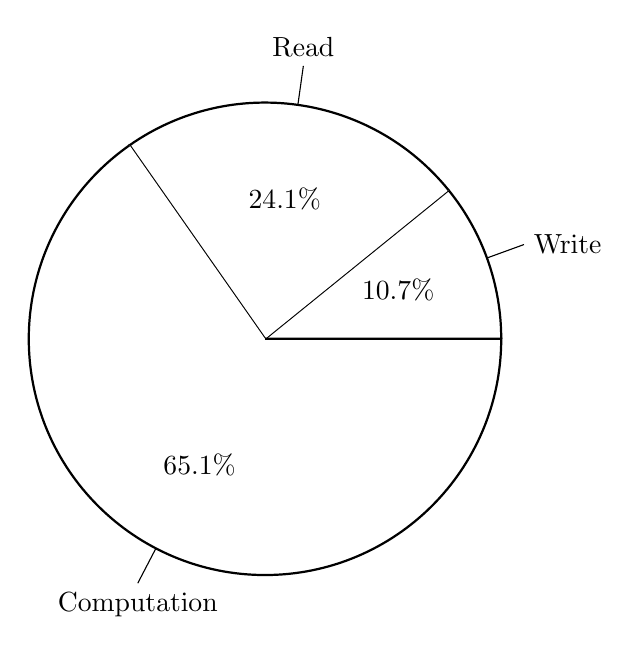
\begin{tikzpicture}
							
							\foreach \start/\end/\middle/\percent/\anchor/\name in {
								0/39/20/10.7/right/Write,
								39/125/82/24.1/above/Read,
								125/360/242.5/65.1/below/Computation}
							{
								\draw[fill=white, thick] (0,0) -- (\end:3cm) arc (\end:\start:3cm)
								node at (\middle:1.8cm) {\textcolor{black}{\percent \%}};
								\draw (\middle:3cm) -- (\middle:3.5cm) node[\anchor] {\name};
							};
							
							\end{tikzpicture}
							\caption{Ratios of time consumed by data transfer versus computation (execution on one core).}
							\label{fig:circle}
						\end{figure}				
						It shows, that the data transfer consumes more than one third of the overall execution time which, is a big drawback. Another peculiarity is that the read time is more than twice the write time. To examine the reasons for that peculiarity, measurements concerning the memory bandwidth had been performed. One idea to explain the low transfer rates was that only a small amount of data was copied. Figure~\ref{fig:bandwidth} shows the measured values of the memory bandwidth for different data sizes.
						\begin{figure}[h]
							\centering
							\begin{tikzpicture}			
							\textit{\begin{axis}[
								width=11cm,
								xmode=log,
								log basis x={2},
								height=7cm,
								log ticks with fixed point,
								scale only axis,
								xmin=1.0, xmax=8193,
								xtick={2,8,32,128,512,2048,8192},
								xlabel={Data [Bytes]},
								xmajorgrids,
								ymin=0.0, ymax=15.1,
								ytick={1,2,3,4,5,6,7,8,9,10,11,12,13,14,15},
								ylabel={Bandwidth [MB/s]},
								ymajorgrids,
								%title={Speedup},
								axis lines*=left,
								%  line width=1.0pt,
								%  mark size=2.0pt,
								legend style ={ at={(0.66,0.18)}, 
									anchor=north west, draw=black, 
									fill=white,align=left},
								cycle list name=black white
								]	
								\addplot[ycomb, mark=square*] table [x=data, y=write, col sep=semicolon] {Messungen/bandwidth.csv};
								\addlegendentry{Bandwidth Write};
								\addplot[ycomb, mark=*] table [x=data, y=read, col sep=semicolon] {Messungen/bandwidth.csv};
								\addlegendentry{Bandwidth Read};					
								\end{axis}}
							\end{tikzpicture}%
							\caption{Measurement of memory bandwidth for different data sizes.}
							\label{fig:bandwidth}
						\end{figure}
						It is shown, that the maximum transfer rate of 15 Megabytes per second is already reached with 128 byte of copied data and the read bandwidth is less than half the write bandwidth. These maximum values are equal to those measured in the implementation. So the reason for the limited transfer rate is not the size of transfered data. Adapteva offers an own bandwidth test. Its output is presented in Figure~\ref{fig:ada_bandwidth}.
						\begin{figure}[h]
							\begin{center}
								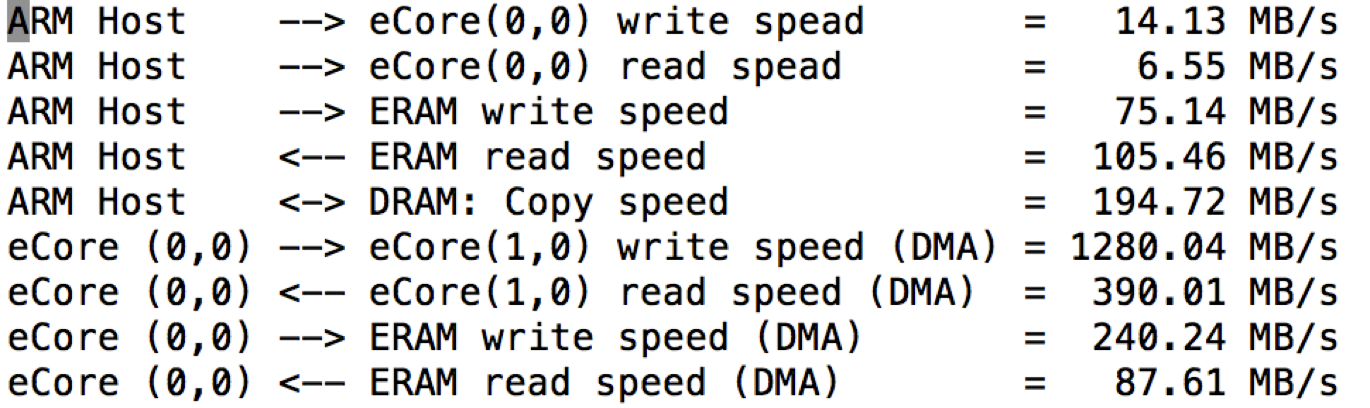
\includegraphics[width=\textwidth]{grafiken/adapteva_bandwidth.png}
								\caption{Results of Adapteva's bandwidth test.}
								\label{fig:ada_bandwidth}
							\end{center}
						\end{figure}
						The first and second values represent the same transfer, from host memory to the Epiphany chip, as performed in Figure~\ref{fig:bandwidth}. Adapteva's measurements are equal to the results of this work. A closer look at the measurements reveals, that there is a different way to achieve a higher memory bandwidth. If you use a special memory, called ERAM, as a temporary storage between host and Epiphany device, a higher transfer rate can be achieved. The memory bandwidth from host memory to ERAM is 75 MB per second for write and 105 MB per second for read transactions. Data copies from ERAM to an Epiphany core result in a transfer rate of 240 MB per second for write and 88 MB/s for read. The results show, that there exists a possibility to reach higher transfer rates. Nevertheless, the results are far from the number presented in Figure~\ref{fig:sysoverview}, where the bandwidth is denoted with 1.4 GB/s for transfers to the Epiphany chip. Furthermore, there is no documentation which explains how to achieve the maximum rates. 
						\begin{figure}[H]
							\centering
							\begin{tikzpicture}			
							\textit{\begin{axis}[
								width=12cm,
								height=6cm,
								scale only axis,
								xmin=1, xmax=4,
								%xtick={Systemmatrix,2,3,4},
								xlabel={number of threads},
								xtick=data,
								%xmajorgrids,
								ymin=0.0, ymax=80,
								ytick={10,20,30,40,50,60,70,80},
								ylabel={time duration [ms]},
								ymajorgrids,
								%title={Speedup},
								axis lines*=left,
								%  line width=1.0pt,
								%  mark size=2.0pt,
								%legend style ={ at={(1,0.2)}, 
								%	anchor=north west, draw=black, 
								%	fill=white,align=left},
								cycle list name=black white,
								ybar,align=center,
								nodes near coords, bar width=25pt,
								enlarge x limits=0.4
								]
								\addplot[fill=tudblue] table[x=threads, y=time, col sep=semicolon]{Messungen/omp.csv};	
								\end{axis}}
							
							\end{tikzpicture}%
							\caption{Time duration of data transfer with OpenMP and variable number of threads.}
							\label{fig:omp}
						\end{figure}
						According to Adapteva's bandwidth test, the memory transfer from host to device should be accelerated by using the ERAM as a temporary memory. Due to technical problems and lack of good documentation, this measure could not be implemented successfully.  
						\\
						Another approach to improve the memory bandwidth is to use OpenMP to parallelize data transfer to the device. Figure~\ref{fig:omp} shows the time improvements that can be achieved by the use of multiple threads. The total transfer time can be reduced by some ten percent if two threads are used. If more than two threads are used, the results are still better compared to the solution with one thread, but there is no further acceleration. 
					\subsection{Performance Measurements}
						To identify bottlenecks and to examine the performance of the implementation, measurements have been done. Table~\ref{tab:meas} gives an overview about the most important measured metrics.
						\begin{table}[h]
							\centering
							\renewcommand{\arraystretch}{1.5}
							\begin{tabular}{|c||r|r|}								
								\hline
													& 1 core	& 16 cores	\\ 
								\hline \hline
								Write Time	& $65$ ms		& $65$ ms \\
								\hline
								Computation Time & $394$ ms & $25$ ms \\
								\hline 
								Read Time	& $146$ ms 	& $148$ ms \\
								\hline
								Number of Floating Point Operations & $13.9 \cdot 10^6$ & $13.9 \cdot 10^6$ \\
								\hline
								MFLOP/s in Computation Part & $35$ MFLOP/s & $556$ MFLOP/s \\
								\hline
								MFLOP/s in Whole Program & 23 MFLOP/s & 57 MFLOP/s \\
								\hline
								Transfer Rate: Write	& $15.4$ MB/s & $15.4$ MB/s \\
								\hline
								Transfer Rate: Read	& $7.01$ MB/s & $6.9$ MB/s \\
								\hline
								\end{tabular}
							\caption{Absolute numbers of measured metrics.}
							\label{tab:meas}
						\end{table}
						Again, the results show that the main bottleneck is the data transfer. Especially in the 16-core version the portion of computation amounts in only ten percent. On the other hand the speedup of the computation part is close to 16 and therefore nearly optimal. If only the computation part is considered, 556~MFLOP/s could be reached, which is about two percent of the theoretical peak performance of the Epiphany chip. The implementation of the FFT includes the calculation of a sine function, that is very time consuming. This measure might be increased, if the sine is replaced by precalculated values in a table. On the other hand the size of local memory and the transfer rates are limited. For this reason, there needs to be a verification if the reduced computation time justifies the increased time for the data transfer of the sine values. The drawbacks could be avoided, if the trigonometric functions would be realized in hardware.
						
						\subsubsection*{Speedup}
						The Speedup of the implementation is calculated according to Formula~\ref{equ:speedup} \cite{Hennesy2012}. $T_\mathrm{1}$ is the time for the serial version and $T_\mathrm{p}$ the time for the parallel execution time with $p$ processors.
						\begin{equation}
							S_\mathrm{p}=\frac{T_\mathrm{1}}{T_\mathrm{p}}
							\label{equ:speedup}
						\end{equation}
						\begin{figure}
							\centering
							\begin{tikzpicture}			
							\textit{\begin{axis}[
								width=11cm,
								height=8cm,
								scale only axis,
								/pgf/number format/use comma,
								xmin=1.0, xmax=16.1,
								xtick={1,2,3,4,5,6,7,8,9,10,11,12,13,14,15,16},
								xlabel={Number of Cores},
								xmajorgrids,
								ymin=1.0, ymax=16.0,
								%ytick={2,3,4,5,6},
								ylabel={Speedup},
								ymajorgrids,
								%title={Speedup},
								axis lines*=left,
								%  line width=1.0pt,
								%  mark size=2.0pt,
								legend style ={ at={(0.6,0.2)}, 
									anchor=north west, draw=black, 
									fill=white,align=left},
								cycle list name=black white
								]	
								\addplot[ycomb, mark=square*] table [x=kerne, y=opt, col sep=semicolon] {Messungen/speedup.csv};
								\addlegendentry{Measured Speedup};
								\addplot[dashed] table [x=kerne, y=kerne, col sep=semicolon] {Messungen/speedup.csv};
								\addlegendentry{Optimal Speedup};					
								\end{axis}}
							\end{tikzpicture}%
							\caption{Speedup of the computation part in comparison with optimal speedup.}
							\label{fig:speedupcalc}
						\end{figure}
						\\
						Figure \ref{fig:speedupcalc} shows the speedup of the computation part in comparison to the optimal speedup. The values could only be measured for multiples of two and three. The Epiphany Software Development Kit offers functions for building groups of threads that work in parallel. These groups can only be rectangular. The cores of the Epiphany are structured in a mesh with four cores in x- and y-dimension. This is the reason why it was not possible with reasonable effort to execute the program with an arbitrary number of cores. Figure \ref{fig:speedupcalc} shows that the measured speedup is nearly linear, if only the computation part is considered. This corresponds to the expected behavior, because there is no communication necessary between the different cores and thus, they do not influence each other.						
						\\
						Figure~\ref{fig:speedupamdahl} shows the speedup of the overall program if the data transfer is considered, too. The data transfer could not be parallelized and therefore the parallel fraction is only 65\%. The optimal speedup according to Amdahl can be calculated according to Formula \ref{equ:amdahl} \cite{Amdahl1967}. 
						\begin{equation}
							S_{pA} = \frac{1}{(1-f)+\frac{1}{p}f}
							\label{equ:amdahl}
						\end{equation}
						$f$ is the parallel fraction, $p$ the number of processors and $S_{pA}$ the speedup according to Amdahl. The maximum speedup according to Amdahl is thus 2.9. Figure~\ref{fig:speedupamdahl} presents the measured values in comparison with the maximum speedup for the number of cores according to Amdahl. Again, the measured values are very close to the calculated optimal speedup. This matches the expected behavior. In the parallel part the cores do not need to communicate or access shared memory locations. This is why the speedup correlates very well with the expectations.
						\begin{figure}[H]
							\centering
							\begin{tikzpicture}			 
							\textit{\begin{axis}[
								width=11cm,
								height=8cm,
								scale only axis,
								/pgf/number format/use comma,
								xmin=1.0, xmax=16.1,
								xtick={1,2,3,4,5,6,7,8,9,10,11,12,13,14,15,16},
								xlabel={Number of Cores},
								xmajorgrids,
								ymin=1.0, ymax=2.6,
								%ytick={2,3,4,5,6},
								ylabel={Speedup},
								ymajorgrids,
								%title={Speedup},
								axis lines*=left,
								%  line width=1.0pt,
								%  mark size=2.0pt,
								legend style ={ at={(0.6,0.2)}, 
									anchor=north west, draw=black, 
									fill=white,align=left},
								cycle list name=black white
								]	
								\addplot[ycomb, mark=square*] table [x=kerne, y=trans, col sep=semicolon] {Messungen/speedup.csv};
								\addlegendentry{Measured Speedup};
								\addplot[dashed] table [x=kerne, y=amdahl, col sep=semicolon] {Messungen/speedup.csv};
								\addlegendentry{Optimal Speedup};					
								\end{axis}}
							\end{tikzpicture}%
							\caption{Overall Speedup in comparison with the optimal speedup according to Amdahl.}
							\label{fig:speedupamdahl}
						\end{figure}
						\clearpage
	\section{Comparison with NVIDIA GeForce GTX 750 Ti}
		\label{sec:gpu}
		In this section the Parallella board is compared with the NVIDIA GeForce GTX 750 Ti in terms of energy efficiency and die size. The architecture of a system with a CPU, the host processor, and a GPU, the device, is similar to the architecture of the Parallella board. There, the host is the ARM processor and the device is the Epiphany chip. 
		\subsection{Maxwell GPU Architecture}
			The Maxwell GPU Architecture is said to have twice the energy efficiency of that of the Kepler GPU architecture due to the new design of the Streaming Multiprocessor (SMM). The new datapath organization and improved instruction scheduler provide more than 40\% higher delivered performance per CUDA core. Figure \ref{fig:smx} shows the Streaming Multiprocessors of Maxwell and Kepler. Immediately it can be seen, that there is a significant difference in the layout between the SMX and the SMM. The SMM is now heavily partitioned. In an SMX the four warp scheduler would share most of their execution resources whereas in an SMM the warp schedulers are removed from each other and given complete dominion over a far smaller collection of execution resources. 
			\begin{figure}[h]		
				\centering
				\begin{subfigure}[b]{0.48\textwidth}
					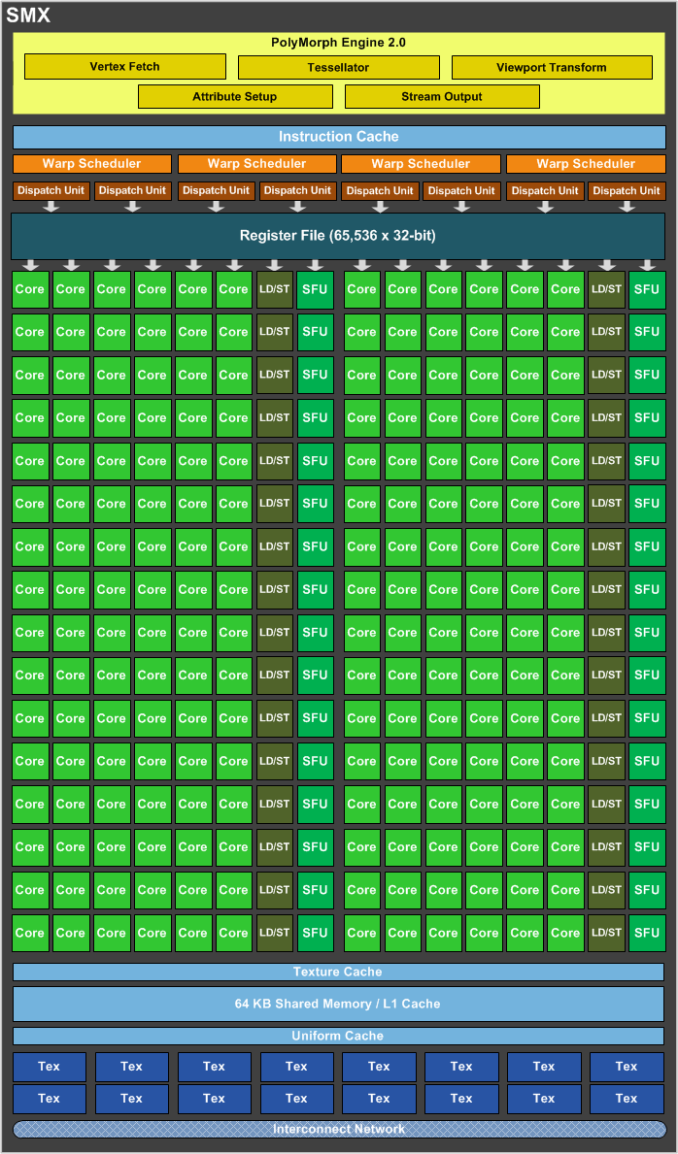
\includegraphics[width=\textwidth]{grafiken/kepler}
					\caption{Kepler Streaming Multiprocessor (SMX)}
				\end{subfigure}
				\begin{subfigure}[b]{0.4347\textwidth}
					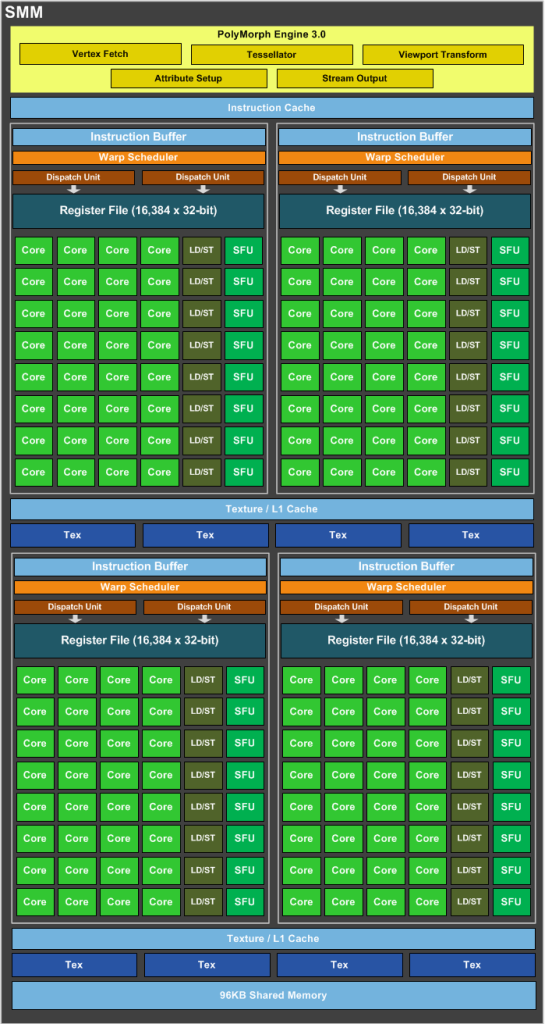
\includegraphics[width=\textwidth]{grafiken/maxwell}
					\caption{Maxwell Streaming Multiprocessor (SMM)}
				\end{subfigure}
				\caption{Block diagram of Kepler and Maxwell Streaming Multiprocessor \cite{Smith2014}.}
				\label{fig:smx}
			\end{figure}Now they do not need to share CUDA cores, load/store units or special function units, because each of them is duplicated in each partition. Besides the goal to achieve better energy efficiency, NVIDIA wanted to increase the space efficiency. The SMM can achieve 92\% of the performance with only 128 cores compared to 192 cores in an SMX.   \cite{Harris2014}\cite{Smith2014}
			
		\subsection{NVIDIA GeForce GTX 750 Ti}
		\label{sec:750}
			The NVIDIA GeForce GTX 750 Ti is one of the first releases of devices with the Maxwell GPU architecture in the high volume market. This GPU includes 5 SMMs with 640 CUDA cores and 2 MB of L2 cache. It is paired with 2 GB of GDDR5-Memory on a 128 Bit bus. 
			\begin{figure}[h]
				\begin{center}
					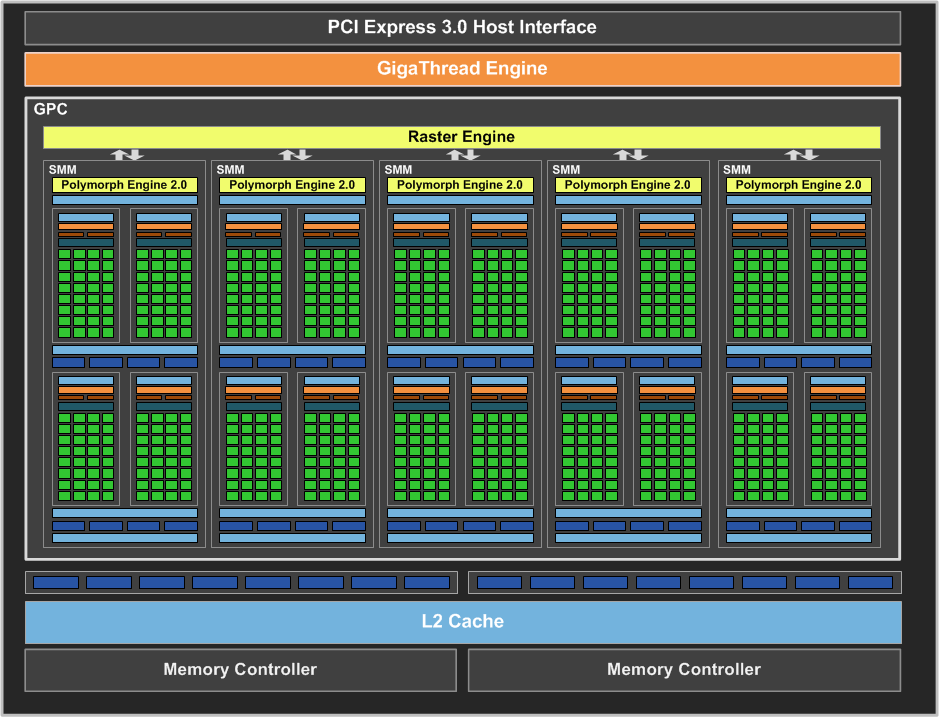
\includegraphics[width=1.0\textwidth]{grafiken/gtx750ti.png}
					\caption{Block diagram of the Nvidia GTX 750 TI \cite{Smith2014}.}
					\label{fig:750ti}
				\end{center}
			\end{figure}
			\\
			The most important specifications of the NVIDIA GeForce GTX 750 Ti are summarized in Table~\ref{tab:speci}. It has a single-precision peak performance of 1,472 TFLOP/s. With a Thermal Design Power of only 60 Watts, the card does not necessarily need an additional power supply and can be fed only by PCI-Express. Nevertheless, many vendors add an additional power supply.\cite{Smith2014}
			\begin{table}[H]
				\centering
				\renewcommand{\arraystretch}{1.2}
				\begin{tabular}{|c|c|}
					\hline Peak Performance Single Precision & 1,472 TFLOP/s \\ 
					\hline Number of SMMs & 5 \\ 
					\hline Number of CUDA cores & 640 \\ 
					\hline Memory Bandwidth  & 86.4 GB/s  \\ 
					\hline Architecture  & Maxwell \\ 
					\hline Memory Bus Interface & 128 Bit \\ 
					\hline Manufacturing Process & TSMC 28nm \\ 
					\hline Thermal Design Power & 60 Watt \\ 
					\hline Launch Date & 02/08/2014 \\ 
					\hline Die size & 148 $mm^2$ \\ 
					\hline 
				\end{tabular}
				\caption{NVIDIA GeForce GTX 750 Ti GPU Specification \cite{Smith2014}.} 
				\label{tab:speci}
			\end{table}
			
			\subsection{Comparison of Parallella and NVIDIA GeForce GTX 750 TI}
				The Epiphany chip and the a GPU are compared in terms of energy efficiency and chip are in this section. The evaluation GPU is a NVIDIA GeForce GTX 750 TI, that was presented in section~\ref{sec:750}. The implementation of the algorithm is the same as presented in Figure~\ref{fig:implementation}. The implementation is based on CUDA, a parallel computing platform and application programming interface developed by NVIDIA. It allows to use a CUDA-enabled GPU for general purpose programming. The FFT is implemented using NVIDIA's cuFFT-Library~\cite{NVIDIA2015}. 
				\subsubsection*{Test Setup}  
				To evaluate the energy efficiency of both the GPU and the Epiphany chip, the Thermal Design power is used. The energy consumption is calculated according to Formula \ref{equ:energy}.
				\begin{equation}
					E = t_\mathrm{runtime} P_\mathrm{TDP}
					\label{equ:energy}
				\end{equation}
				$t_\mathrm{runtime}$ is the runtime of the computation part of the implementation and $P_\mathrm{TDP}$ is the Thermal Design Power. The Thermal Design Power of the 16-core Epiphany is 2 Watts respectively 60 Watts for the NVIDIA GeForce GTX 750 Ti. Of course, the use of the Thermal Design Power is a simplification, but it was not possible to measure the energy consumption more precisely with reasonable effort. The function \mintinline{c}{clock_gettime} measures the execution times.
				\subsubsection*{Energy efficiency}
					For the following examinations, only the computation part of the algorithm is considered. If the data transfer is taken into account, too, a fair comparison is not possible. The transfer rate of the Parallella is not comparable to those from CPU to GPU via PCI-Express. Thus, the following results are only valid under the assumption, that only the computation part is considered.
					\begin{table}[]
						\centering
						\renewcommand{\arraystretch}{1.2}
						\begin{tabular}{|c|c|c|}
							\hline
							Number of Pictures & Parallella & GPU \\
							\hline\hline
							1 & 50 mJ & 10,200 mJ \\
							\hline
							100  & 50 mJ & 114 mJ \\
							\hline 
							1000 & 50 mJ & 35 mJ \\
							\hline
							5000 & 50 mJ & 26 mJ \\
							\hline
							10000 & 50 mJ & 25 mJ \\
							\hline
						\end{tabular}
						\caption{Energy consumption per Picture of the Parallella and GPU implementation.}
						\label{tab:energy}
					\end{table}
					\\
					In Table~\ref{tab:energy} the energy consumption per picture of the Parallella and GPU implementation are presented. The Parallella is already completely utilized with one picture, and thus the energy consumption per picture stays constant. On the other hand, the measurements show that the energy consumption per picture of the GPU implementation improves, if the number of pictures increases. If only one picture is calculated, the Parallella clearly outperforms the GPU in terms of energy efficiency. The reason is, that the initialization phase of cuFFT is very time consuming and the GPU is not utilized entirely. If more pictures are computed, the GPU beats the Parallella and provides a lower energy consumption per picture. The implementation on the Parallella can be improved, if for example the time consuming computation of the sine function is removed or further improvement techniques like loop unrolling are used. It can be stated, that in this implementation the energy consumption per picture is better on the GPU for a big amount of pictures and can be achieved with lower effort. On the other hand the Parallella implementation can be improved and thus, the energy consumption per picture. The optimization is more challenging compared to the GPU, due to the limited documentation and local memory size. Furthermore, the manufacturing process needs to be considered. The Epiphany is a 65 nm chip, whereas the GPU is manufactured in 28 nm. For this reason, the energy efficiency of the Epiphany improves, if the manufacturing process would be 28 nm. 
					
				\subsubsection*{Energy efficiency of a 1024-core Epiphany chip}  
					In this section an example configuration of Adapteva for an Epiphany chip with 1024 cores \cite{Olofsson2011}, shall be compared to the GPU. Table~\ref{tab:1024} shows the specification of that chip. 
					Due to the equal manufacturing process of 28 nm and the similar die size, both the 1024-core Epiphany and the GPU (Table \ref{tab:speci}) are comparable to each other.
					\begin{table}[H]
						\centering
						\renewcommand{\arraystretch}{1.2}
						\begin{tabular}{|c|c|}
							\hline
							Number of cores & 1024 \\
							\hline
							Manufacturing Process & 28 nm \\
							\hline
							Max. Operating Frequency & 700 MHz \\
							\hline
							Peak Performance (Single Precision) & 1,408 GFLOP/s \\
							\hline
							Die Size & 131 $mm^2$ \\
							\hline
							Thermal Design Power & 20 Watt \\
							\hline
						\end{tabular}
						\caption{Specification of an example configuration of an Epiphany chip with 1024 cores \cite{Olofsson2011}.}
						\label{tab:1024}
					\end{table}
					The energy efficiency is approximately six times better than that of the 16-core Epiphany used in this work. There, the energy efficiency per picture would be better than that of the GPU.  
	\clearpage
	\section{Conclusion}
		In this work the Adapteva Parallella board was presented. In the first section the architecture and specification of the board, as well as the structure of the Epiphany chip were shown. On this basis, the FFT algorithm was implemented. Furthermore, the performance was examined and the data transfer from host to device was analyzed in detail. Finally, the implementation was repeated for the NVIDIA GeForce GTX 750 Ti. Both solutions were compared to each other in terms of energy efficiency.
		\\
		The results show, that the Parallella is very affordable. For only 99\$ you get a credit card-sized stand-alone computer or an embedded device. This is the reason why this tool is nice for gathering experience in parallel programming. Institutions or interested people could buy this hardware at low cost and practice parallel programming. The Epiphany chip is energy efficient. Any core has its own small sized local memory, that is no managed cache; the user has full control over this memory. This is an advantage compared to architectures with a hardware managed cache, because you can optimize and control the access to that very fast memory. On the other hand the developer has more responsibilities and needs to put more effort into its memory accesses. Additionally there is no cache coherency latency. Especially for a large amount of cores this produces a large overhead, e. g. the Intel Xeon Phi \cite{Fang2013}.
		\\
		On the other hand, the main disadvantage for real high-speed applications is the data transfer bottleneck. Due to the limited local memory size, for code as well as data, small memory transfers from host to device are necessary and should be as quick as possible. The measurements in this work show, that data transfer is time consuming and the main bottleneck. Furthermore, the Parallella has a small user base and an expandable documentation. For this reason, it is hard to do a good implementation in reasonable time and for beginners, a good documentation is essential, too.
		\\
		All in all, the Adapteva Parallella is a board that is not yet ready for serious high-performance implementations. It might be well suited as an entrance to parallel programming, but for this a better documentation and support is necessary. The Epiphany is a good idea and an efficient architecture. It is unclear, if Adapteva's story can continue, but probably the ideas will live on in newer architectures.
	\clearpage
	\nocite{*}
	\printbibliography[heading=bibintoc]
\end{document}